\section{Problema 3 - Canal RAGB: \texorpdfstring{$M$}{M}-QAM}

Considerando que um sinal ($s_m$) de mensagem passa por um canal de Ruído Adivitivo Gaussiano Branco (RAGB), um modelo como uma variável aleatoria Gaussiana complexa, como na equação~\ref{fig:4QAM_25dB}. O sinal foi recebeido no filtro casado e é dado por

\begin{figure}[!ht]
    \centering
    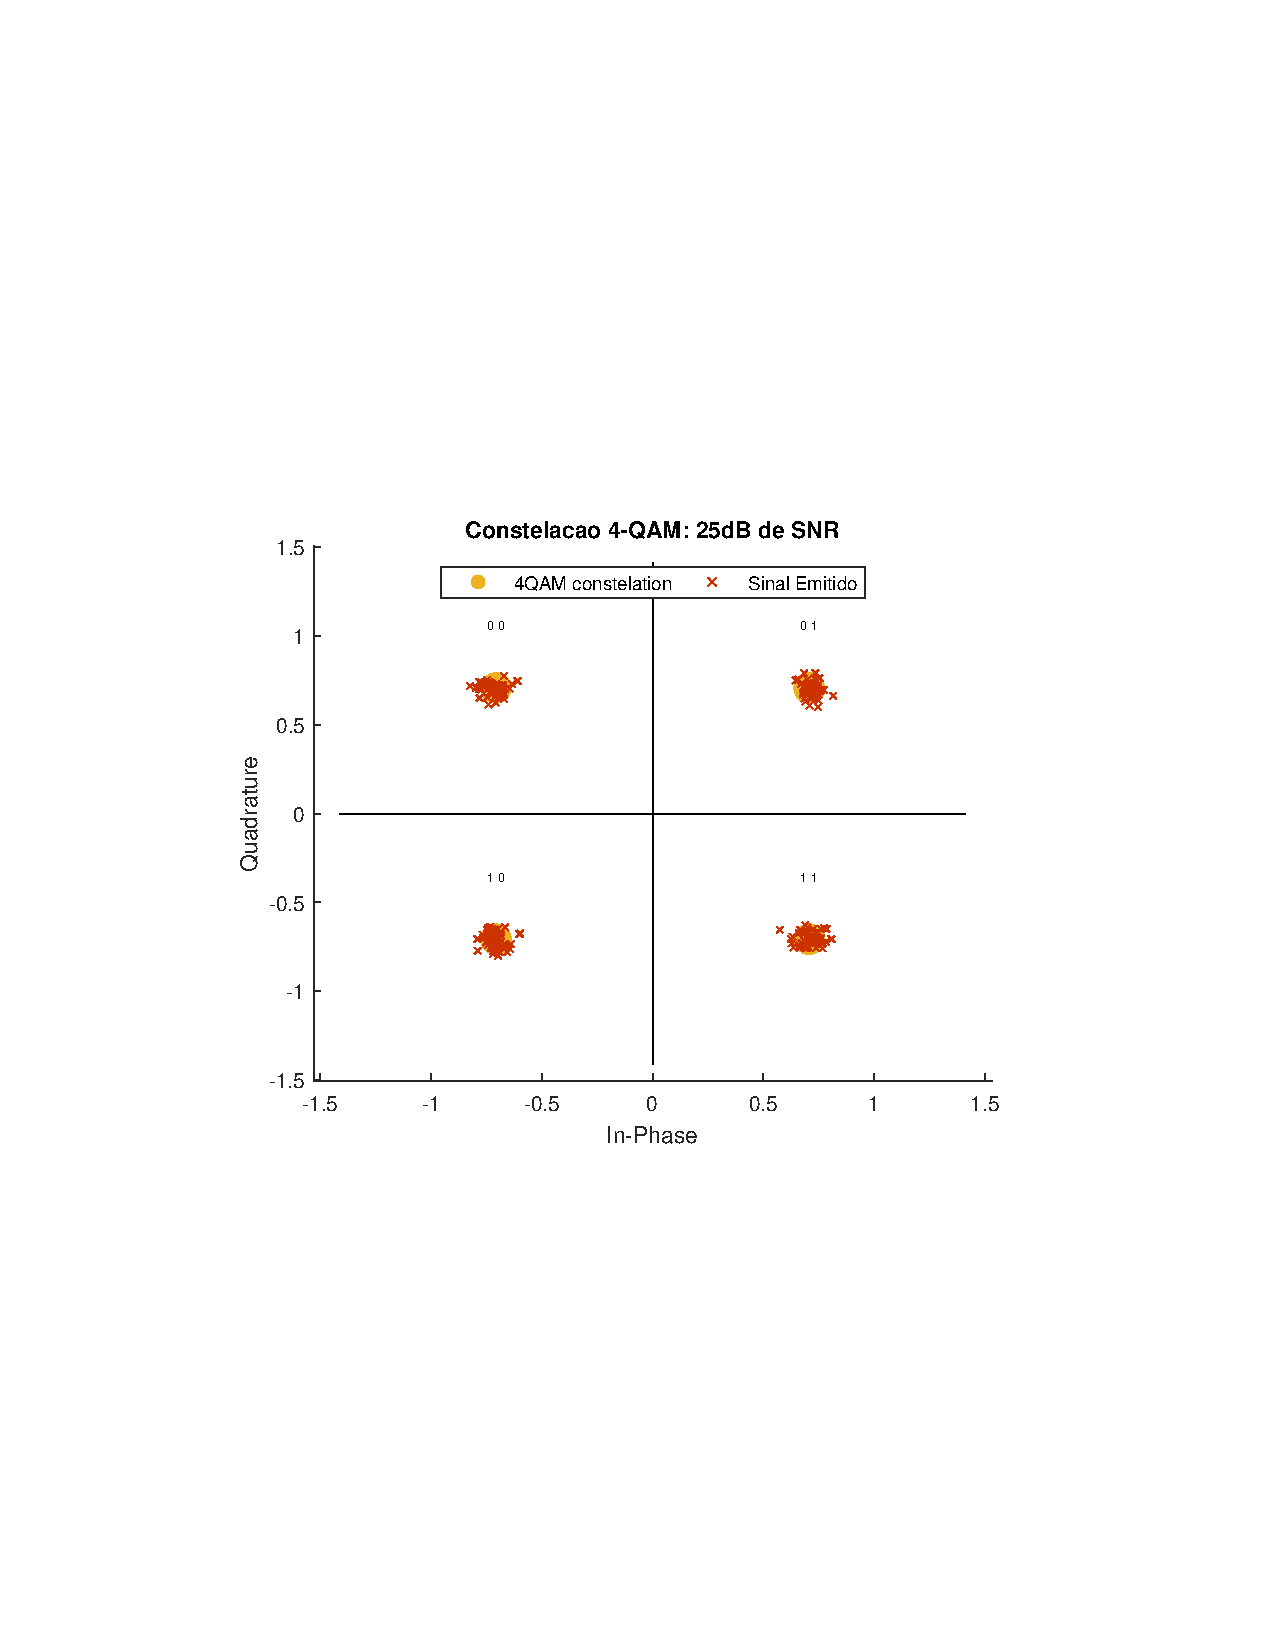
\includegraphics[width=1.0\textwidth,clip=true,trim={1.5cm 8.5cm 1.8cm 8.3cm}]{C:/Users/lukin/Documents/GitHub/Courses-HWs/Sistemas de Comunicacoes Digitais/matlab/problema3/fig/4QAM_25dB.pdf}
    \caption{Simulação de transmissão $4$-QAM, com \textit{SNR} de 25dB.}
    \label{fig:4QAM_25dB}
\end{figure}

Para o caso de $16$-QAM

\begin{figure}[!ht]
    \centering
    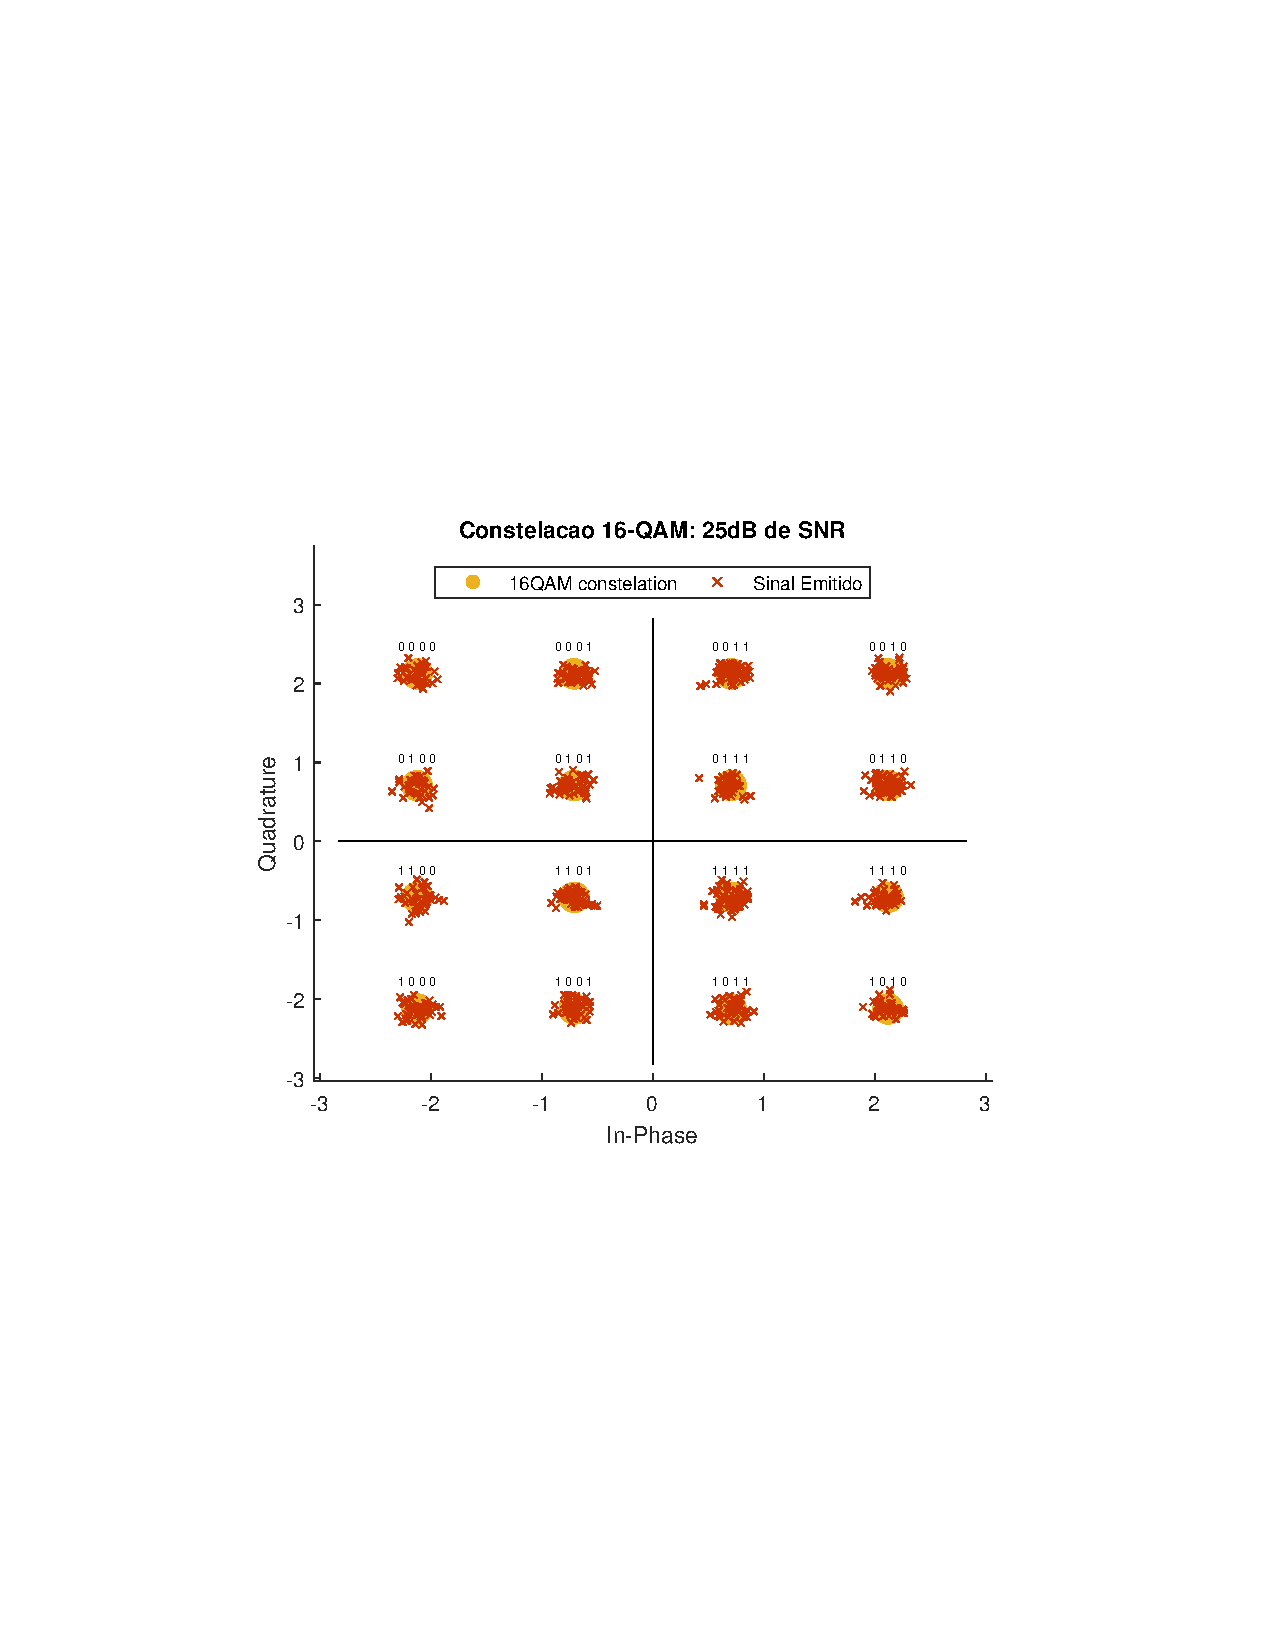
\includegraphics[width=1.0\textwidth,clip=true,trim={1.5cm 8.5cm 1.8cm 8.3cm}]{C:/Users/lukin/Documents/GitHub/Courses-HWs/Sistemas de Comunicacoes Digitais/matlab/problema3/fig/16QAM_25dB.pdf}
    \caption{Simulação de transmissão $16$-QAM, com \textit{SNR} de 25dB.}
    \label{fig:16QAM_25dB}
\end{figure}

\begin{figure}[!ht]
    \centering
    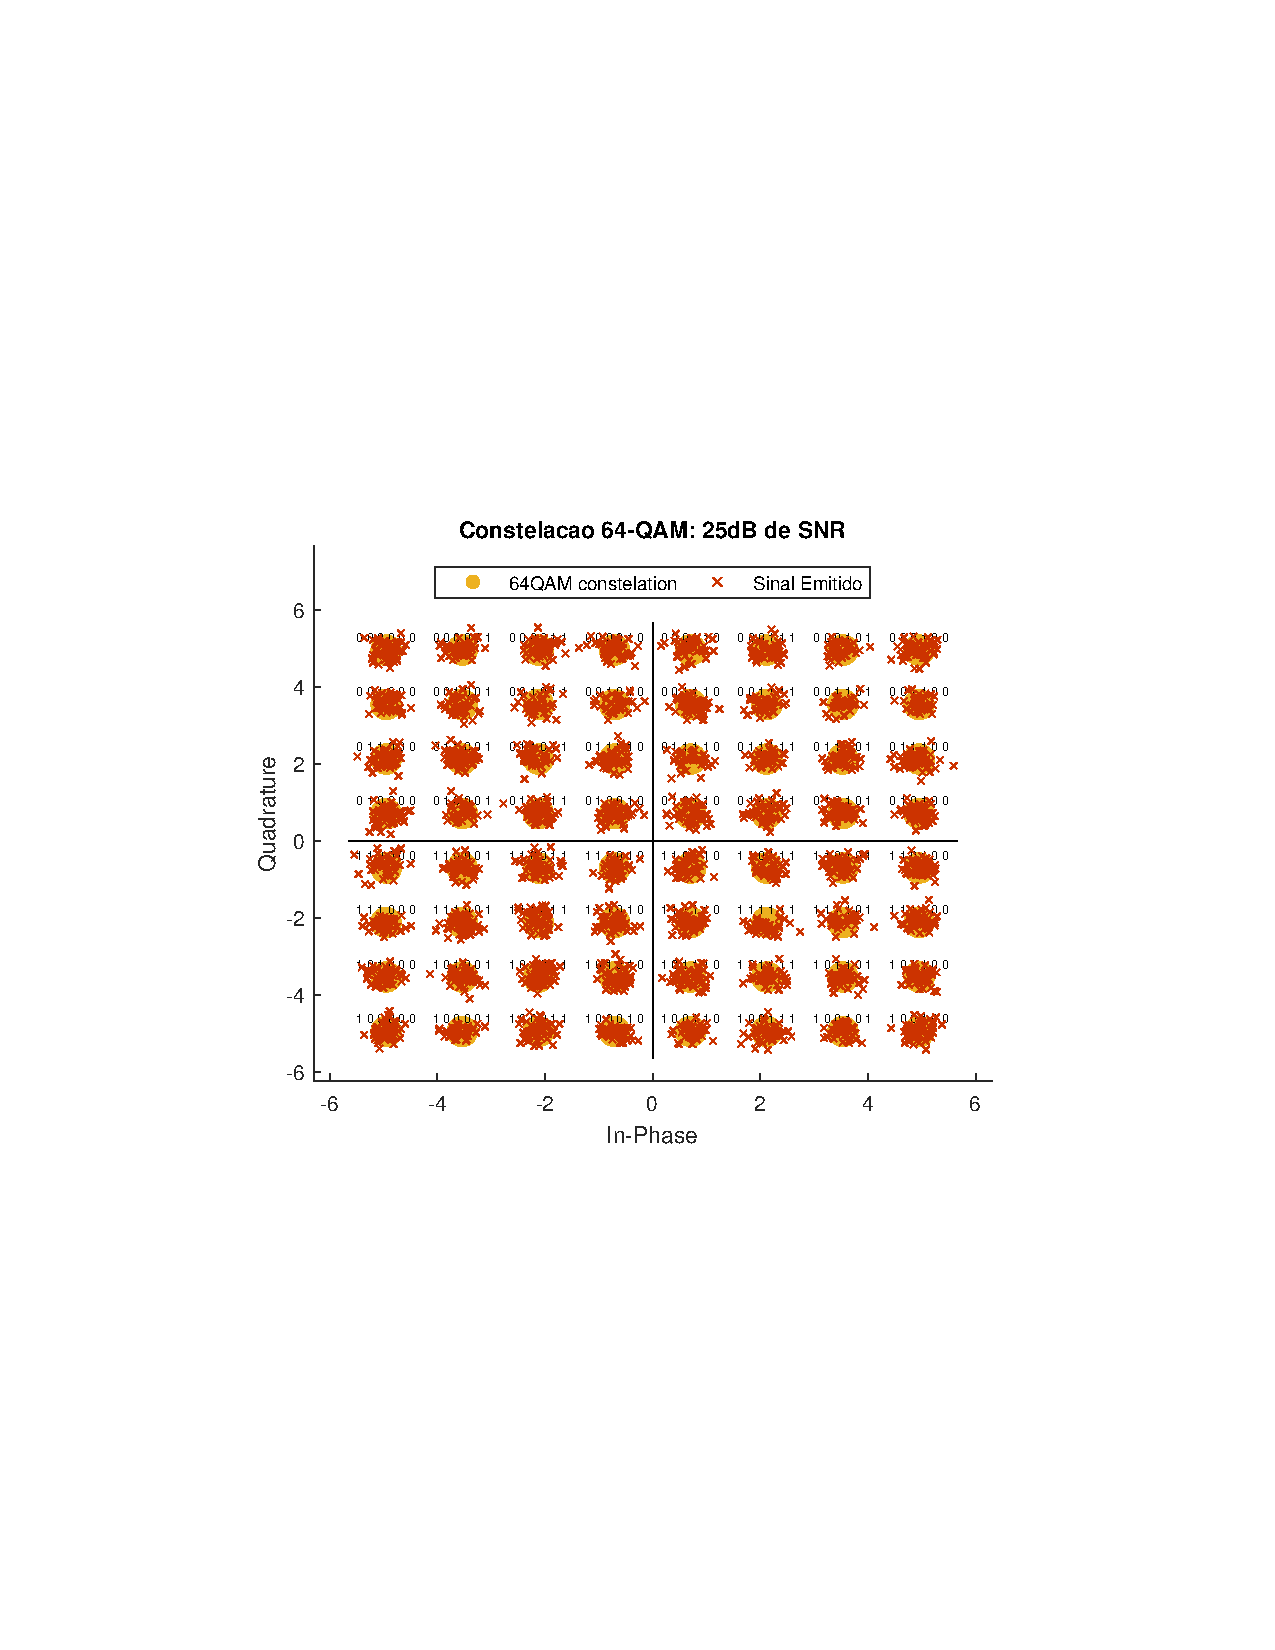
\includegraphics[width=1.0\textwidth,clip=true,trim={1.5cm 8.5cm 1.8cm 8.3cm}]{C:/Users/lukin/Documents/GitHub/Courses-HWs/Sistemas de Comunicacoes Digitais/matlab/problema3/fig/64QAM_25dB.pdf}
    \caption{Simulação de transmissão $64$-QAM, com \textit{SNR} de 25dB.}
    \label{fig:64QAM_25dB}
\end{figure}


\begin{figure}[!ht]
    \centering
    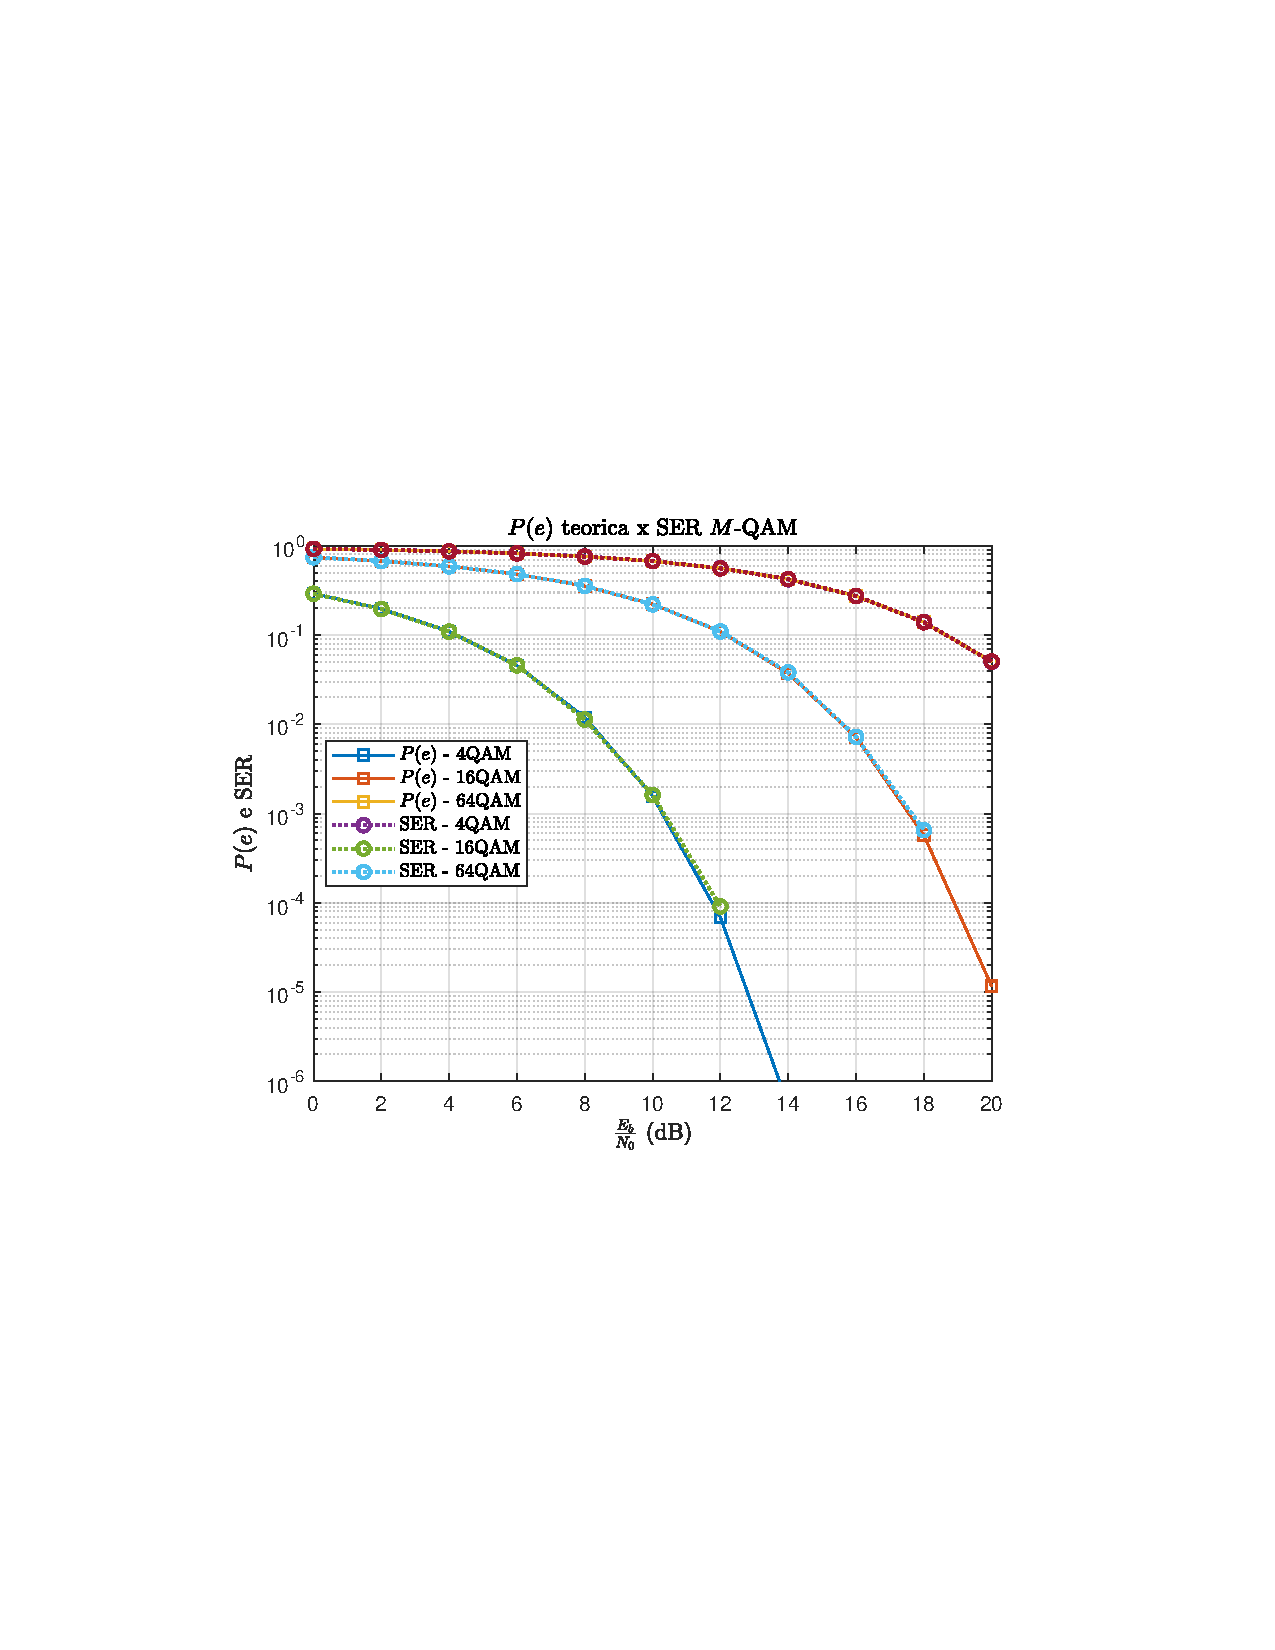
\includegraphics[width=1.0\textwidth,clip=true,trim={1.5cm 8.5cm 1.8cm 8.3cm}]{C:/Users/lukin/Documents/GitHub/Courses-HWs/Sistemas de Comunicacoes Digitais/matlab/problema3/fig/Erro_teoricaxAWGN_MQAM.pdf}
    \caption{Probabilidade teórica de erro vs. simulação de transmissão $M$-QAM em canal RAGB.}
    \label{fig:Erro_teoricaxAWGN_MQAM}
\end{figure}